\documentclass[lettersize,journal]{IEEEtran}
% TGRS 正式投稿须改为英文全文；本稿为中文技术定稿草稿，版式按 IEEEtran journal（与 TGRS 一致）。
% Overleaf / 本地请使用 XeLaTeX。
\usepackage{xeCJK}
\usepackage{amsmath,amssymb,amsfonts}
\usepackage{algorithmic}
\usepackage{algorithm}
\usepackage{array}
\usepackage{booktabs}
\usepackage{multirow}
\usepackage{tabularx}
\usepackage{graphicx}
\usepackage{cite}
\usepackage{url}
\usepackage{textcomp}
\usepackage{stfloats}
\usepackage{xcolor}
\usepackage{balance}
\graphicspath{{./images/}}
\hyphenation{op-tical net-works semi-conduc-tor IEEE-Xplore}

% 仍缺内容：红色占位（定稿/投稿前删除本宏及全部调用）
\newcommand{\ExpTodo}[2]{%
  \textcolor{red}{\textbf{【待补-#1】}}%
  \textcolor{red}{（#2）}%
}

\begin{document}

\title{面向边缘部署的红外弱小目标检测可迁移压缩框架}

\author{Guotai Sun, Qin Shu%
\thanks{\ExpTodo{Affil}{作者单位、通信作者邮箱、基金号按最终投稿信息填写。}}}

\markboth{IEEE Transactions on Geoscience and Remote Sensing,~Vol.~XX, No.~XX, Month~20XX}%
{Sun \MakeLowercase{\textit{et al.}}: Transferable Compression Framework for Edge IRSTD}

\maketitle

\begin{abstract}
红外弱小目标检测（infrared small-target detection, IRSTD）在预警监视、安防与遥感中具有重要价值。深度学习显著提升了检测精度，但高精度模型参数与计算开销大，难以直接部署到以 Rockchip RK3588 为代表的嵌入式平台。现有路线或从零设计轻量网络，或采用通用/任务剪枝，却仍主要依赖权重大小、小波能量等代理指标，且往往缺少跨骨干统一协议与板端实测闭环。
本文提出与具体检测骨干解耦的可迁移压缩框架：（1）将任意 IRSTD 分割网络映射为统一剪枝组；（2）融合目标区域加权损失梯度与局部对比先验的小目标敏感性评分，并按尺度分层配额；（3）在共掩码约束下结构化收缩通道宽度并拷贝教师权重；（4）以区域分割损失与输出蒸馏重训恢复，再导出 ONNX/RKNN 做板端评估。
在 DNA-Net、UIU-Net、MSHNet 与 SCTransNet 上，纯 CNN 骨干学生相对教师 Params 下降约 $72\%$--$78\%$、FLOPs 下降约 $54\%$--$62\%$；SCTransNet 因仅收缩 CNN 宽度，Params/FLOPs 约 $-49.5\%$/$34.2\%$。四骨干 IoU 与统一脚本目标级 $P_d$/$F_a$ 总体保持；RK3588 延迟下降约 $12\%$--$39\%$，且算力下降并不等比转化为墙钟加速。进一步在相近 Params 下对照从零轻量网络表明：难集（NUAA-SIRST、SIRST-V2）上从零轻量明显弱于压缩学生，而易集可打平，从而支撑“压缩高精度骨干以继承难集能力”的动机。
\end{abstract}

\begin{IEEEkeywords}
Infrared small-target detection, model compression, channel pruning, knowledge distillation, embedded deployment, transferable framework, RK3588
\end{IEEEkeywords}

%==============================================================================
\section{引言}
\label{sec:intro}
\IEEEPARstart{单}{帧}红外弱小目标检测旨在从单幅红外图像中定位尺寸极小、对比度弱、纹理匮乏的目标\cite{DNANet2023,ACM2021}。与可见光通用检测不同，目标往往仅占极少像素，并易被云层、海杂波与地物纹理淹没，对特征保持与背景抑制要求极高。

近年来，DNA-Net\cite{DNANet2023}、UIU-Net\cite{UIUNet2023}、MSHNet\cite{MSHNet2024} 与 SCTransNet\cite{SCTransNet2024}等显著提升了公开基准上的交并比（IoU）、检测概率 $P_d$ 与虚警率 $F_a$。然而精度提升常伴随参数量、浮点运算与访存增长，使模型难以部署到算力与功耗受限的边缘平台。工程上，纸面 Params/FLOPs 下降也并不等价于 NPU 真实加速：算子支持、带宽与运行时调度共同决定可用性。

现有高效化研究大致两类。一类从零设计轻量网络\cite{RDIAN2023,LWIRSTNet2023,RepISDNet2023,L2SKNet2025}，结构紧凑，但容量上限有限，在真实难场景上易掉点。另一类对高精度模型做压缩：IRPruneDet\cite{IRPruneDet2024} 引入小波结构正则软通道剪枝；SAGCP\cite{SAGCP2025} 以稀疏编码诱导冗余通道删除。二者证明了 IRSTD 需要专用剪枝，但仍存在不足：（i）重要性多为权重/稀疏代理，与检测指标对齐不充分；（ii）跨 CNN/Transformer 的统一压缩协议不完整；（iii）效率评价偏 GPU 上的 Params/FLOPs，板端证据不足。

本文将贡献定位为\textbf{可迁移压缩协议}，而非某一改结构的检测器变体：
\begin{enumerate}
\item 提出面向 IRSTD 的小目标敏感性评分，融合目标区域加权任务梯度与局部对比先验，并由浅层保护、深层多剪的分层配额导出保留通道。
\item 给出与骨干解耦的剪枝组抽象与共掩码结构化压缩：拓扑（跳连/嵌套/Transformer 层数）保持不变，仅收缩宽度；各骨干仅实现 Adapter。
\item 固定区域分割损失与输出知识蒸馏重训配方，使“继承高容量教师判别能力”成为可检验命题。
\item 在 DNA-Net、UIU-Net、MSHNet 与 SCTransNet 上验证协议泛化，并在 RK3588 上闭环评估 Params/FLOPs、RKNN 体积、延迟、进程 RSS 与 NPU 忙碌时间估计；同时以相近 Params 的从零轻量网络做\textbf{难集}对照，解释为何选择压缩而非仅依赖从零轻量结构。
\end{enumerate}

本文其余部分：第~\ref{sec:related}~节相关工作；第~\ref{sec:method}~节方法；第~\ref{sec:exp}~节实验；第~\ref{sec:concl}~节结论。

%==============================================================================
\section{相关工作}
\label{sec:related}

\subsection{红外弱小目标检测}
传统方法包括滤波、局部对比与低秩稀疏分解等\cite{IPI2013}，可解释性强但对复杂场景鲁棒性有限。深度学习将任务建模为像素级分割：ACM/ALCNet\cite{ACM2021,ALCNet2021}引入上下文与局部对比；DNA-Net\cite{DNANet2023}以密集嵌套维持深层小目标响应；UIU-Net\cite{UIUNet2023}采用 U-Net in U-Net；ISNet\cite{ISNet2022}强调形状；MSHNet\cite{MSHNet2024}以尺度--位置敏感损失配合简洁多尺度头；SCTransNet\cite{SCTransNet2024}引入空间嵌入的通道式 Transformer。上述高精度模型构成本文压缩的教师起点与泛化验证对象。

\subsection{轻量网络与嵌入式部署}
RDIAN\cite{RDIAN2023}、RepISD-Net\cite{RepISDNet2023}、L$^2$SKNet\cite{L2SKNet2025}、LW-IRSTNet\cite{LWIRSTNet2023}等从结构设计阶段控制复杂度，后者还报告了开发板推理速度。该类工作是相近 Params 下的从零轻量精度基线；本文则强调从高容量模型压缩并继承难集能力，并以师生板端闭环验证部署收益，而非与从零轻量做板端竞速。

\subsection{模型压缩与 IRSTD 专用剪枝}
通用剪枝如 Network Slimming\cite{NetworkSlimming2017}、Soft Filter Pruning\cite{SoftFilterPruning2018}等面向分类，易误伤 IRSTD 所需浅层空间细节。IRPruneDet\cite{IRPruneDet2024}、SAGCP\cite{SAGCP2025} 证明了任务专用剪枝的必要性。知识蒸馏\cite{HintonDistill2015}为剪后恢复提供通用工具。本文差异在于：面向小目标的区域敏感评分、跨架构共掩码协议、蒸馏恢复与板端效率闭环一体。

%==============================================================================
\section{方法}
\label{sec:method}

\subsection{问题形式化}
\label{sec:problem}
给定已训练的 IRSTD 分割教师 $M_T$、精度容差 $\varepsilon$ 与复杂度/延迟预算 $B$，目标是得到学生 $M_S$，使得
\begin{equation}
\label{eq:obj}
\mathrm{Acc}(M_S)\ge \mathrm{Acc}(M_T)-\varepsilon,\qquad
\mathrm{Cost}(M_S)\le B,
\end{equation}
其中 $\mathrm{Acc}$ 采用 IoU（及 $P_d$、$F_a$），$\mathrm{Cost}$ 可为 Params、FLOPs 与板端延迟。关键约束是：压缩协议应尽量与 $M_T$ 的具体拓扑解耦。

\subsection{总体框架}
\label{sec:overview}
如图~\ref{fig:pipeline}所示，框架含四步：
Adapter 枚举剪枝组 $\rightarrow$
小目标敏感性评分 $\rightarrow$
结构化压缩与权重拷贝 $\rightarrow$
蒸馏重训与板端部署。

\begin{figure*}[!t]
\centering
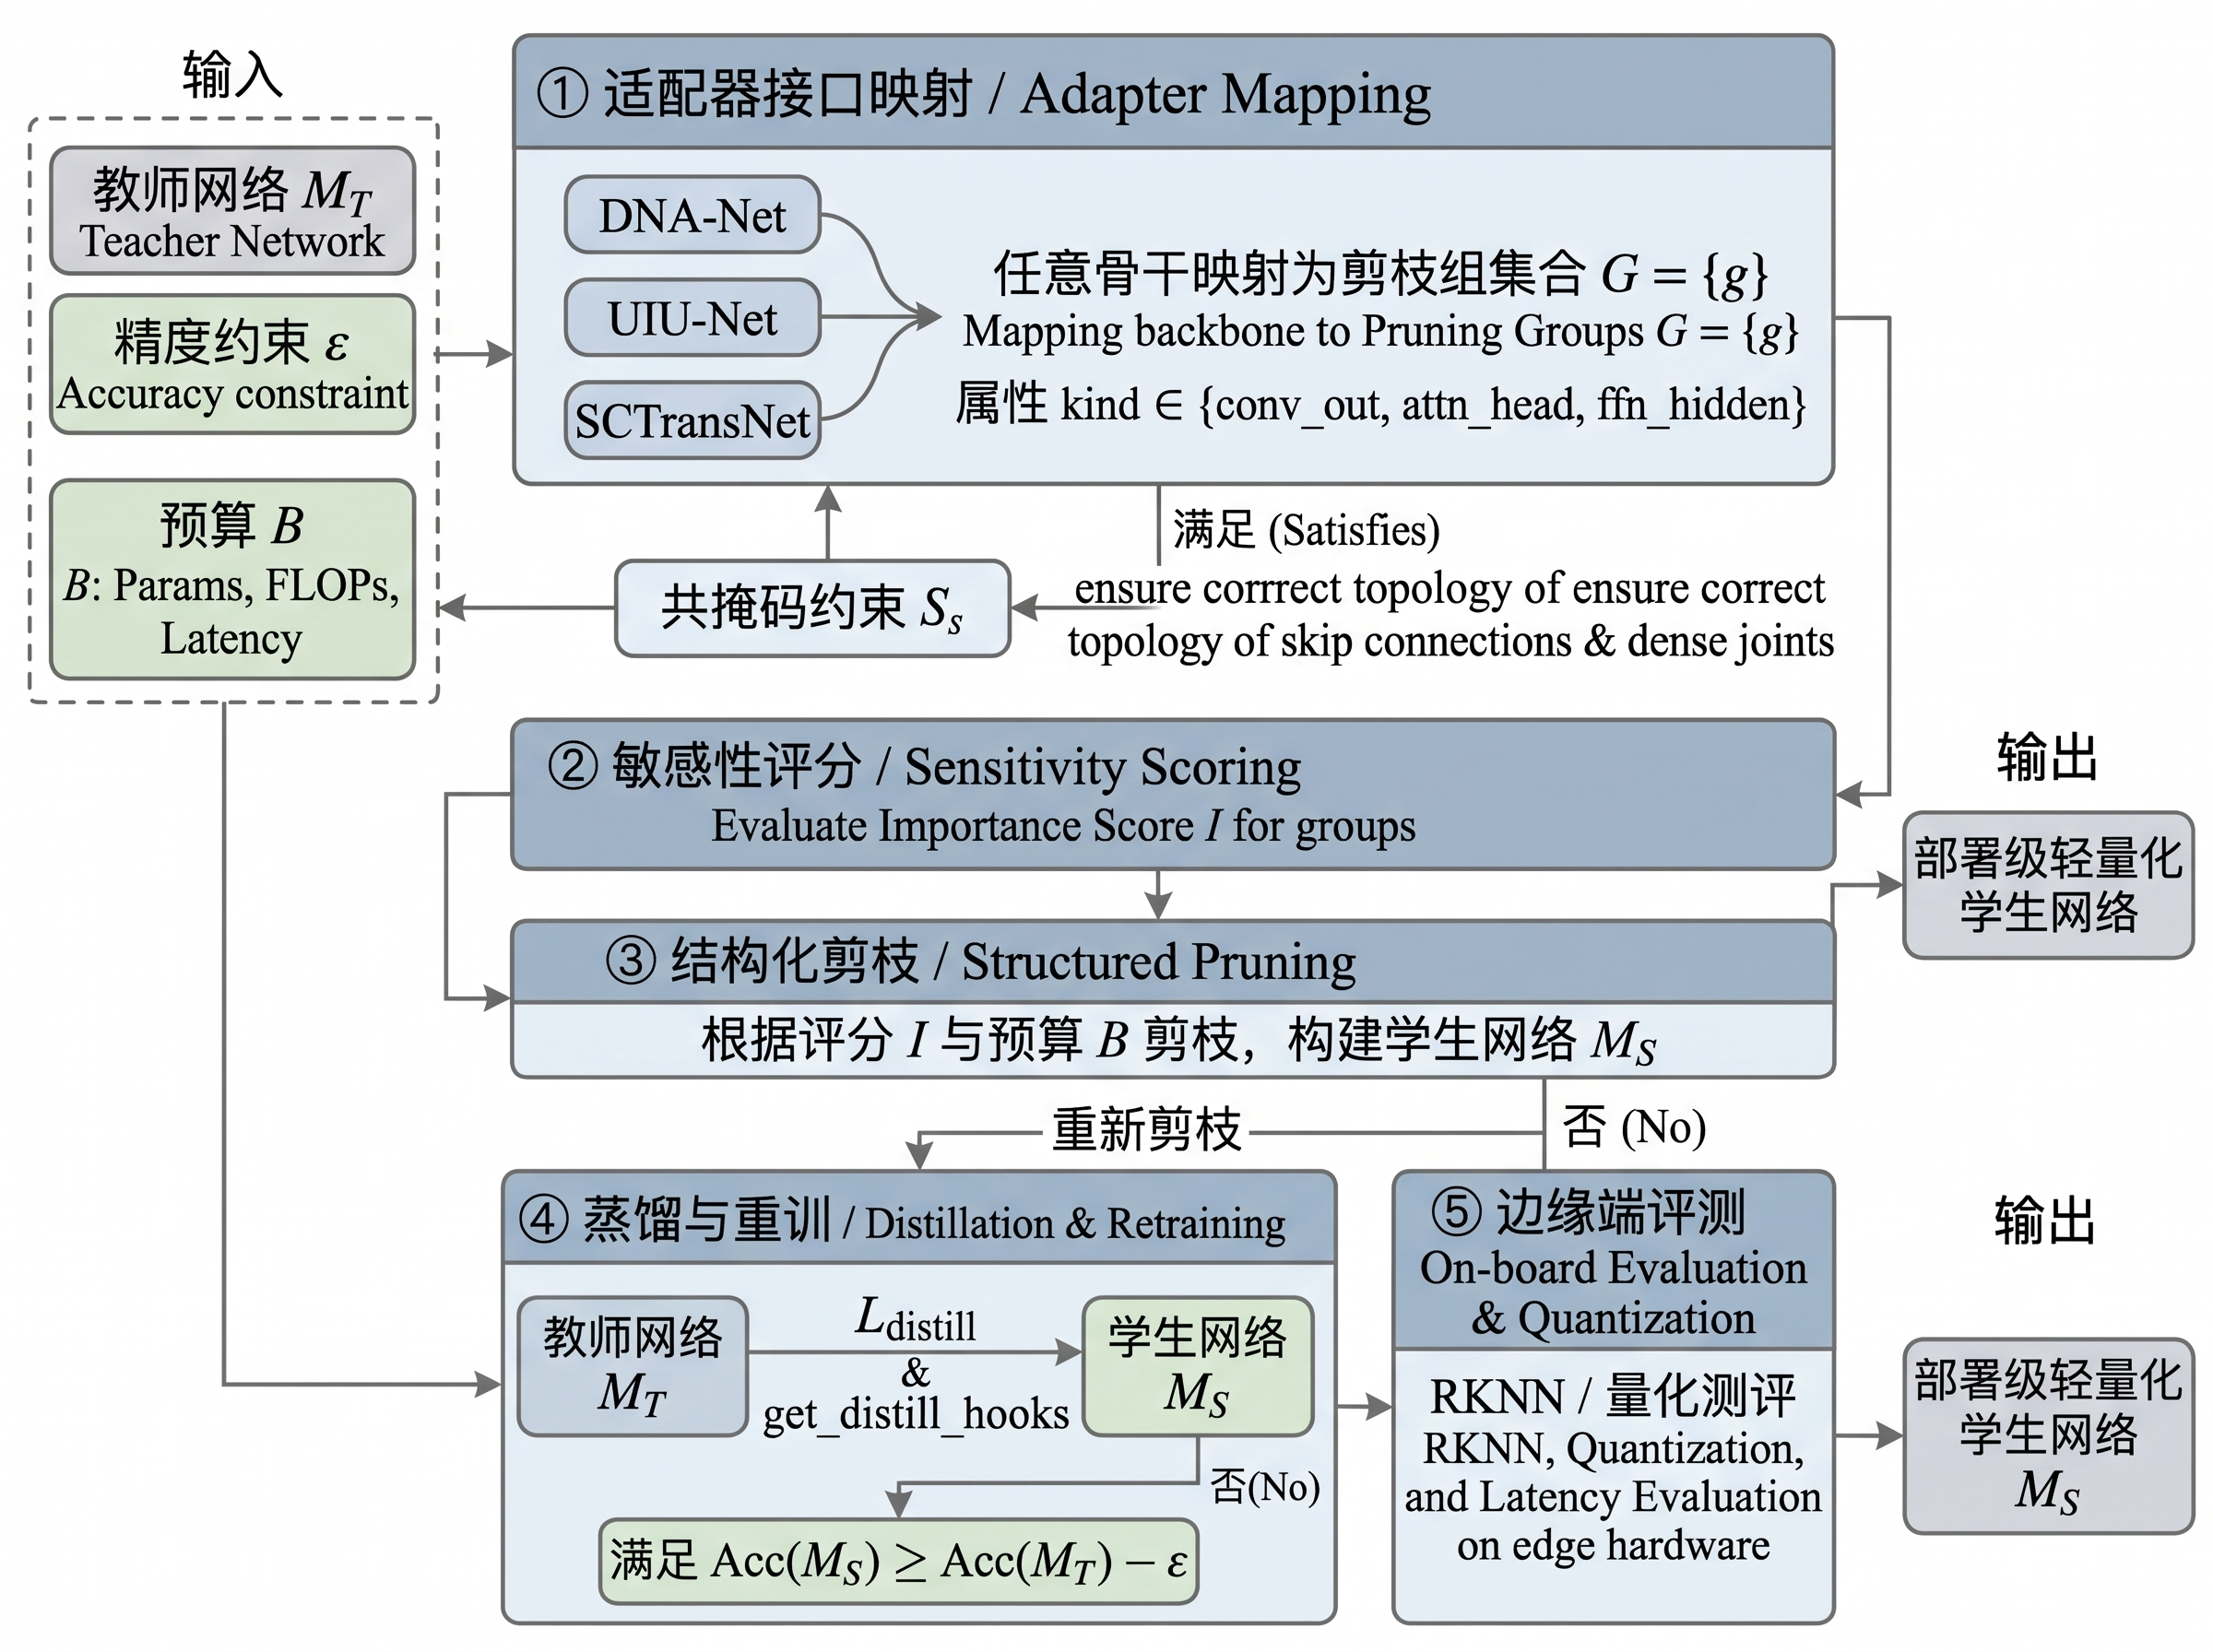
\includegraphics[width=0.92\textwidth]{fig1.png}
\caption{所提可迁移压缩框架总体流程：Adapter 映射、敏感性评分、共掩码结构化变窄、蒸馏恢复与 RK3588 部署评估。}
\label{fig:pipeline}
\end{figure*}

\subsection{剪枝组抽象与模型适配}
\label{sec:adapter}
将任意骨干映射为剪枝组集合 $\mathcal{G}=\{g\}$。每个组包含：类型（实现以 $\mathrm{conv\_out}$ 为主）、阶段编号 $\mathrm{stage\_id}$、可剪通道数 $C_g$，以及需同步切片的模块集合。

\textbf{共掩码约束：}对存在跳跃连接或密集拼接的尺度 $s$，所有输出宽度同为该尺度通道维的组共享同一保留下标集合 $S_s$。该约束保证 DNA-Net 嵌套节点、UIU-Net/MSHNet 跳连、SCTransNet 编解码拼接在变窄后仍拓扑合法。

每个骨干仅实现适配器：\texttt{enumerate\_groups}、\texttt{build\_student}（含权重切片）及评分用特征/梯度钩子。评分、配额、蒸馏与导出主体不随模型复制。实例化见表~\ref{tab:adapter}。

\begin{table}[!t]
\renewcommand{\arraystretch}{1.15}
\caption{骨干 Adapter 实例化（与实现一致）}
\label{tab:adapter}
\centering
\begin{tabular}{@{}p{2.2cm}p{5.4cm}@{}}
\toprule
骨干 & 剪枝组要点 \\
\midrule
DNA-Net & 5 档 \texttt{nb\_filter}；尺度共掩码；Res-CBAM 同步切片 \\
MSHNet & 5 档 \texttt{param\_channels}；Res+CBAM 同步切片 \\
UIU-Net & 4 档 stage 宽度；RSU 拓扑不变；mid 通道按比例缩放 \\
SCTransNet & 4 档 CNN 宽度；\texttt{KV\_size}$=\sum$ 通道；Transformer \textbf{层数/头数不变} \\
\bottomrule
\end{tabular}
\end{table}

\subsection{小目标敏感性评分}
\label{sec:importance}
对组 $g$ 的第 $c$ 个输出通道，定义
\begin{equation}
\label{eq:I}
I(g,c)=\alpha\,\hat{I}_{\mathrm{task}}(g,c)+(1-\alpha)\,\hat{I}_{\mathrm{contrast}}(g,c),
\end{equation}
其中 $\hat{\cdot}$ 表示组内 min-max 归一化，默认 $\alpha=0.7$。

\textbf{任务项 $I_{\mathrm{task}}$：}
采用目标区域加权 SoftIoU：在真值 mask 的膨胀邻域内计算损失并对教师反传，取残差块末层卷积权重梯度幅值，按输出通道聚合，再在若干训练 batch 上平均，以减轻背景像素主导。

\textbf{对比项 $I_{\mathrm{contrast}}$：}
记组输出特征为 $A$，则
\begin{equation}
\label{eq:contrast}
I_{\mathrm{contrast}}(g,c)=\mathbb{E}\!\big[\bar{A}_{c}^{\mathrm{tgt}}-\bar{A}_{c}^{\mathrm{bg}}\big],
\end{equation}
即目标邻域平均响应与背景平均响应之差，体现红外局部对比先验。

\textbf{分层配额：}
按 $\mathrm{stage\_id}$ 设定剪枝率 $p_s$（浅层小、深层大）。五尺度默认 $p=(0.2,0.3,0.4,0.5,0.6)$，四尺度 CNN 为 $(0.2,0.3,0.4,0.5)$。
对 SCTransNet，因 Transformer 层数/头数不变、压缩空间主要来自 CNN 宽度，采用更温和配额 $p=(0.05,0.15,0.25,0.35)$，并强制偶数通道以兼容分组卷积。
组内按 $I$ 降序保留约 $(1-p_s)C_g$ 个通道。
为避免耗时的硬件在环搜索，将式~\eqref{eq:obj} 中预算 $B$ 实例化为经验分层配额 $\{p_s\}$；纯 CNN 单次压缩约可削减 $55\%$--$60\%$ FLOPs，SCTransNet 约 $34\%$。若已知具体板端延迟预算，可在该配额邻域做轻量网格或二分校准，而不改变协议主体。

\textbf{可选校准：}
Top-$k$/Bottom-$k$ 通道敲除曲线可与 $\ell_1$、随机剪枝对照，以加强 $I$ 的因果解释。
主文以表~\ref{tab:criterion}与图~\ref{fig:criterion}的同压缩率准则对照为实测证据；逐步敲除曲线见图~\ref{fig:knockout}。
\ExpTodo{Knockout}{图~\ref{fig:knockout} 现为示意形态；请用 GPU 逐步敲除实测 CSV 替换后重绘。}

\subsection{结构化压缩}
\label{sec:prune}
在配额 $\{p_s\}$ 下得到 $\{S_s\}$，重建更窄学生 $M_S$，并将教师卷积/BN（及注意力中与通道绑定的参数）按索引切片拷贝。硬约束：同 stage 共掩码；BN 统计量同步；分割头输出维不剪。过程不修改跳连/嵌套/Transformer 层数语义，仅改变宽度。

\subsection{蒸馏重训与板端部署}
\label{sec:distill}
剪后优化目标为
\begin{equation}
\label{eq:loss}
\begin{aligned}
\mathcal{L}=&\ 
\lambda_{\mathrm{seg}}\,\mathcal{L}_{\mathrm{seg}}(M_S,y)
+\lambda_{\mathrm{region}}\,\mathcal{L}_{\mathrm{region}}(M_S,y)\\
&+\lambda_{\mathrm{kd}}\,\mathcal{L}_{\mathrm{KD}}\!\big(M_S(x),M_T(x)\big),
\end{aligned}
\end{equation}
其中 $\mathcal{L}_{\mathrm{seg}}$ 为各骨干习惯的分割损失（SoftIoU/BCE 及多尺度头），$\mathcal{L}_{\mathrm{region}}$ 为目标区域加权 SoftIoU，$M_T$ 冻结；$\mathcal{L}_{\mathrm{KD}}$ 为输出掩膜 MSE（logits 经 sigmoid 或教师已输出概率）。默认 $\lambda_{\mathrm{seg}}=\lambda_{\mathrm{kd}}=1$，$\lambda_{\mathrm{region}}=0.5$（SCTransNet 取 $0.75$）；DNA-Net/UIU-Net/MSHNet 蒸馏约 $200$ epoch，SCTransNet 约 $350$ epoch。

板端导出固定分辨率 ONNX，经 rknn-toolkit2 转为 RKNN，在 RK3588 上测量延迟、进程 RSS、NPU 负载，并估计忙碌时间 $\approx\mathrm{latency}\times\mathrm{mean(NPU\%)}$。评分决定“剪谁”，板端决定“是否真快”，二者解耦。

\begin{algorithm}[!t]
\caption{可迁移 IRSTD 压缩协议}
\label{alg:main}
\begin{algorithmic}
\STATE \textbf{输入：}教师 $M_T$，数据 $\mathcal{D}$，预算 $B$ 的实例化配额 $\{p_s\}$，蒸馏轮数 $E$
\STATE $\mathcal{G}\leftarrow \texttt{Adapter.enumerate\_groups}(M_T)$
\STATE 在 $\mathcal{D}$ 上计算 $I(g,c)$（式~\eqref{eq:I}）；按 $\{p_s\}$ 生成 $\{S_s\}$
\STATE $M_S\leftarrow \texttt{Adapter.build\_student}(M_T,\{S_s\})$；切片拷贝权重
\STATE 按式~\eqref{eq:loss} 蒸馏 $E$ 轮，保存验证集最佳学生
\STATE 导出 ONNX/RKNN；板端测评
\STATE \textbf{输出：}$M_S$
\end{algorithmic}
\end{algorithm}

%==============================================================================
\section{实验}
\label{sec:exp}

\subsection{实验设置}
\label{sec:setup}

\subsubsection{数据集与协议}
采用 NUAA-SIRST、NUDT-SIRST、IRSTD-1k 与 SIRST-V2，划分遵循各数据集官方或社区常用的 \texttt{trainval.txt}/\texttt{test.txt}。训练分辨率以各教师默认为主：DNA-Net/MSHNet/SCTransNet 常用 $256\times256$；UIU-Net 与官方一致，教师与学生蒸馏采用 rescale $320$、随机 crop $288$，表~\ref{tab:main_iou} 中 UIU 的 IoU 亦在同一评测管线（测试 rescale $320$、无 crop）下统计。表~\ref{tab:resource} 的 RK3588 资源对比统一在 $256\times256$ 下测量，该设定仅用于板端效率，不改变精度表分辨率协议。

\subsubsection{评价指标}
精度以 IoU 为主；目标级 $P_d$、$F_a$ 为补充。
$P_d$/$F_a$ 由统一脚本对教师与学生复测：概率图阈值 $0.5$ 二值化，连通域质心距离 $<3$ 判为命中；$P_d$ 为命中目标数/GT 目标数，$F_a$ 为未匹配预测像素数/全图像素数。
效率：Params(M)、FLOPs(G，$\approx 2\times$MACs)、RKNN 体积(MB)；板端：延迟 mean(ms)、进程 RSS mean、估计 NPU 忙碌 ms/帧（非功率计）。

\subsubsection{实现细节}
PyTorch 训练；敏感性评分默认 $50$ batch，$\alpha=0.7$，膨胀核半径 $3$。DNA-Net/UIU-Net/MSHNet 蒸馏默认 $200$ epoch，SCTransNet $350$ epoch；DNA-Net/MSHNet 优化器与教师一致（常用 Adagrad），UIU-Net/SCTransNet 常用 Adam。板端：RK3588，librknnrt $2.5.0$，\texttt{core\_mask}$=7$，warmup $20$、iters $80$，输入 $1\times256\times256\times3$（SCTransNet 为单通道灰度）。随机种子 $42$。

\subsubsection{对比与定位}
\begin{itemize}
\item \textbf{主对比：}同骨干教师 vs 学生，验证压缩有效且可迁移；板端资源表仅覆盖师生（表~\ref{tab:resource}）。
\item \textbf{外部动机对照（H1）：}相近 Params 下，比较从零轻量网络与 DNA-Net 教师/学生在\textbf{难集}（NUAA-SIRST、SIRST-V2）上的 IoU；NUDT-SIRST 与 IRSTD-1k 一并报告。此处为分集训练后的难集容量对照，而非跨数据集零样本迁移。
\item \textbf{剪枝族参照：}IRPruneDet\cite{IRPruneDet2024} 作相关工作参照；SAGCP\cite{SAGCP2025} 无公开权重，仅引用摘要相对压缩量，不做逐格 IoU 硬比。
\end{itemize}

\subsection{主结果：精度}
\label{sec:main_results}

表~\ref{tab:main_iou}给出教师/学生 best IoU。总体结论：\textbf{压缩后 IoU 未系统性下降}。UIU-Net 与 MSHNet 师生基本持平（均值差约 $0.02$--$0.15$ 个百分点），个别数据集略降（如 MSHNet 在 IRSTD-1k/SIRST-V2）。SCTransNet 学生均值由 $0.7907$ 变为 $0.7858$（约 $-0.49$ 个百分点），NUAA/NUDT 略升，IRSTD-1k/SIRST-V2 略降，整体仍处持平区间。

DNA-Net 上学生均值由 $0.7250$ 升至 $0.7696$，涨幅高于其余骨干。解释如下，而非仅归因于“蒸馏偶然增益”：（1）DNA-Net 原生五层密集嵌套在 NUAA/NUDT 等小样本集上存在过参数化，结构化变窄相当于强结构正则；（2）学生重训额外使用 $\mathcal{L}_{\mathrm{region}}$，强化边界与小目标收敛，而教师原始训练未使用该区域项。
用与学生相同评测脚本对 DNA-Net 教师复测，IoU 与表~\ref{tab:main_iou}一致，排除口径伪差。表~\ref{tab:distill}进一步表明：仅 GT 重训已超过教师，区域损失继续增益，涨点主要由结构正则与区域项驱动。

\begin{table}[!t]
\renewcommand{\arraystretch}{1.12}
\caption{教师 vs 学生 best IoU（四数据集）}
\label{tab:main_iou}
\centering
\begin{tabular}{@{}lccccc@{}}
\toprule
方法 & NUAA & NUDT & IRSTD-1k & SIRST-V2 & 均值 \\
\midrule
DNA-Net 教师 & 0.7171 & 0.8488 & 0.6230 & 0.7112 & 0.7250 \\
本文-DNA 学生 & 0.7387 & 0.9226 & 0.6706 & 0.7464 & 0.7696 \\
\midrule
UIU-Net 教师 & 0.7686 & 0.8596 & 0.6376 & 0.8558 & 0.7804 \\
本文-UIU 学生 & 0.7741 & 0.8471 & 0.6439 & 0.8625 & 0.7819 \\
\midrule
MSHNet 教师 & 0.6909 & 0.7558 & 0.6779 & 0.7320 & 0.7142 \\
本文-MSH 学生 & 0.6959 & 0.7729 & 0.6653 & 0.7220 & 0.7140 \\
\midrule
SCTransNet 教师 & 0.7765 & 0.9444 & 0.6685 & 0.7735 & 0.7907 \\
本文-SCTrans 学生 & 0.7849 & 0.9524 & 0.6437 & 0.7620 & 0.7858 \\
\bottomrule
\end{tabular}
\end{table}

表~\ref{tab:main_pdfa}给出统一脚本下的 $P_d$/$F_a$。四骨干学生 $P_d$ 均值均不低于教师；多数设置 $F_a$ 持平或下降。少数设置 $F_a$ 升高（如 UIU/MSH/SCTrans 在 IRSTD-1k），但伴随 $P_d$ 上升或 IoU 仅小幅波动，不构成系统性虚警恶化。

\begin{table*}[!t]
\renewcommand{\arraystretch}{1.12}
\caption{统一脚本下的教师/学生 $P_d$（$\uparrow$）与 $F_a$（$\downarrow$）。阈值 $0.5$，质心匹配距离 $<3$}
\label{tab:main_pdfa}
\centering
\begin{tabular}{@{}lccccc@{}}
\toprule
方法 & NUAA & NUDT & IRSTD-1k & SIRST-V2 & 均值 $P_d$ \\
\midrule
DNA 教师 & $0.9633$/$3.90\!\times\!10^{-6}$ & $0.9873$/$1.34\!\times\!10^{-5}$ & $0.9116$/$9.41\!\times\!10^{-6}$ & $0.8867$/$6.38\!\times\!10^{-6}$ & 0.9372 \\
DNA 学生 & $0.9908$/$3.90\!\times\!10^{-6}$ & $0.9767$/$3.15\!\times\!10^{-6}$ & $0.9320$/$7.59\!\times\!10^{-6}$ & $0.9400$/$9.18\!\times\!10^{-6}$ & 0.9599 \\
\midrule
UIU 教师 & $1.0000$/$1.70\!\times\!10^{-6}$ & $0.9862$/$5.03\!\times\!10^{-6}$ & $0.9044$/$6.80\!\times\!10^{-6}$ & $0.9333$/$3.59\!\times\!10^{-6}$ & 0.9560 \\
UIU 学生 & $1.0000$/$2.61\!\times\!10^{-6}$ & $0.9810$/$6.79\!\times\!10^{-6}$ & $0.9488$/$1.79\!\times\!10^{-5}$ & $0.9333$/$3.09\!\times\!10^{-6}$ & 0.9658 \\
\midrule
MSH 教师 & $1.0000$/$6.44\!\times\!10^{-5}$ & $0.9407$/$2.35\!\times\!10^{-5}$ & $0.9320$/$9.79\!\times\!10^{-6}$ & $0.9267$/$9.60\!\times\!10^{-6}$ & 0.9498 \\
MSH 学生 & $0.9817$/$4.67\!\times\!10^{-5}$ & $0.9598$/$1.66\!\times\!10^{-5}$ & $0.9422$/$2.00\!\times\!10^{-5}$ & $0.9267$/$5.42\!\times\!10^{-6}$ & 0.9526 \\
\midrule
SCTrans 教师 & $0.9450$/$6.64\!\times\!10^{-5}$ & $0.9915$/$2.53\!\times\!10^{-6}$ & $0.9327$/$1.21\!\times\!10^{-5}$ & $0.9333$/$7.43\!\times\!10^{-7}$ & 0.9506 \\
SCTrans 学生 & $0.9817$/$1.40\!\times\!10^{-5}$ & $0.9915$/$3.10\!\times\!10^{-6}$ & $0.9562$/$3.10\!\times\!10^{-5}$ & $0.9467$/$1.11\!\times\!10^{-6}$ & 0.9690 \\
\bottomrule
\end{tabular}
\end{table*}

图~\ref{fig:pareto}给出精度--复杂度 Pareto：各骨干由教师到学生沿 Params/FLOPs 轴左移，同时均值 IoU 基本保持或上升。

\begin{figure}[!t]
\centering
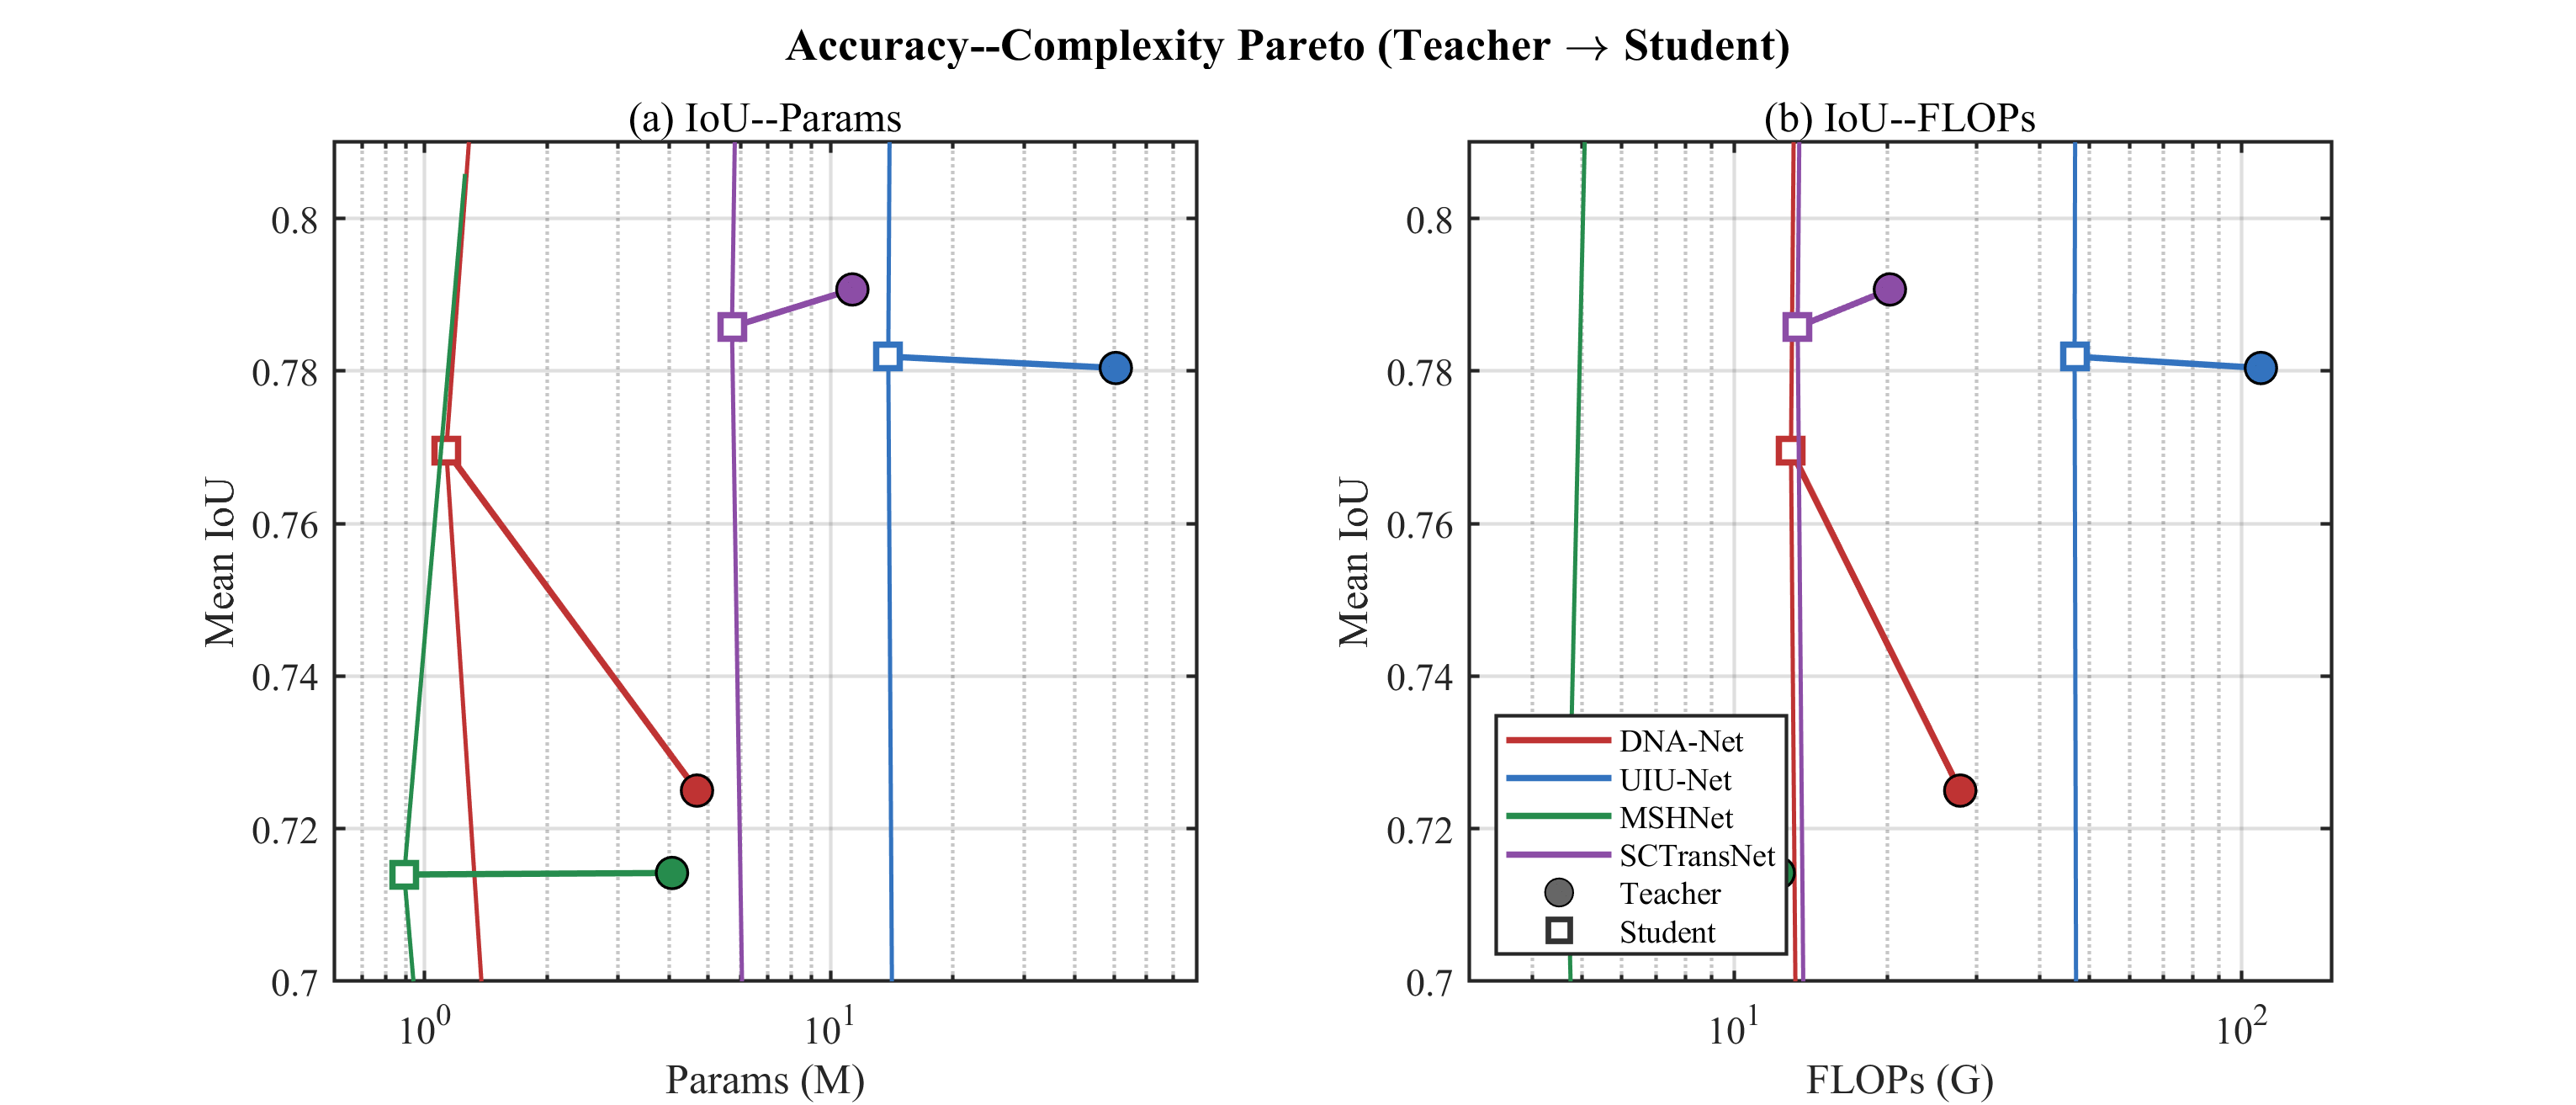
\includegraphics[width=\columnwidth]{fig_pareto.png}
\caption{精度--复杂度 Pareto：各骨干教师（实心）到学生（空心）的压缩轨迹。左：Mean IoU--Params；右：Mean IoU--FLOPs（横轴对数）。复杂度取自 NUAA@$256$ 资源表。}
\label{fig:pareto}
\end{figure}

\subsection{复杂度与板端资源}
\label{sec:edge}

表~\ref{tab:resource}汇总四骨干在 NUAA-SIRST、$256\times256$、RK3588 上的闭环结果。可观察：
\begin{itemize}
\item 纯 CNN（DNA/UIU/MSH）Params 降约 $72\%$--$78\%$，FLOPs 降约 $54\%$--$62\%$；SCTransNet 因 Transformer 未剪，Params/FLOPs 约 $-49.5\%$/$34.2\%$；
\item RKNN 体积均显著下降；墙钟延迟有收益，但\textbf{降幅通常小于 FLOPs 降幅}（DNA、SCTrans 尤为明显）；
\item 估计 NPU 忙碌时间在 DNA/MSH 上近似持平，UIU 与 SCTrans 上下降更明显。
\end{itemize}

\begin{table*}[!t]
\renewcommand{\arraystretch}{1.12}
\caption{NUAA-SIRST、$256\times256$、RK3588 资源对比（教师 $\rightarrow$ 学生）。延迟/RSS 为 \texttt{resource\_bench}，$80$ iters}
\label{tab:resource}
\centering
\begin{tabular}{@{}lcccccc@{}}
\toprule
骨干 & Params (M) & FLOPs (G) & RKNN (MB) & 延迟 mean (ms) & RSS mean (MB) & NPU busy (ms/帧) \\
\midrule
DNA-Net & $4.69\!\rightarrow\!1.13$ & $27.85\!\rightarrow\!12.92$ & $14.6\!\rightarrow\!8.0$ & $1034\!\rightarrow\!913$ & $90.7\!\rightarrow\!80.5$ & $249\!\rightarrow\!256$ \\
 & (\textbf{$-75.8\%$}) & (\textbf{$-53.6\%$}) & ($-45\%$) & (\textbf{$-11.7\%$}) & ($-11.2\%$) & ($\approx$持平) \\
\midrule
UIU-Net & $50.54\!\rightarrow\!13.89$ & $109.0\!\rightarrow\!46.8$ & $113.8\!\rightarrow\!34.7$ & $658.9\!\rightarrow\!404.3$ & $198.0\!\rightarrow\!110.8$ & $309\!\rightarrow\!221$ \\
 & (\textbf{$-72.5\%$}) & (\textbf{$-57.1\%$}) & (\textbf{$-69.5\%$}) & (\textbf{$-38.6\%$}) & (\textbf{$-44.1\%$}) & (\textbf{$-28.3\%$}) \\
\midrule
MSHNet & $4.07\!\rightarrow\!0.89$ & $12.22\!\rightarrow\!4.70$ & $10.58\!\rightarrow\!4.43$ & $478.9\!\rightarrow\!374.2$ & $59.6\!\rightarrow\!53.0$ & $105\!\rightarrow\!100$ \\
 & (\textbf{$-78.2\%$}) & (\textbf{$-61.5\%$}) & (\textbf{$-58.1\%$}) & (\textbf{$-21.9\%$}) & ($-11.1\%$) & ($\approx$持平) \\
\midrule
SCTransNet & $11.33\!\rightarrow\!5.72$ & $20.24\!\rightarrow\!13.32$ & $36.4\!\rightarrow\!22.7$ & $236.2\!\rightarrow\!202.4$ & $87.4\!\rightarrow\!65.7$ & $117.1\!\rightarrow\!98.3$ \\
 & (\textbf{$-49.5\%$}) & (\textbf{$-34.2\%$}) & (\textbf{$-37.8\%$}) & (\textbf{$-14.3\%$}) & (\textbf{$-24.8\%$}) & (\textbf{$-16.1\%$}) \\
\bottomrule
\end{tabular}
\end{table*}

\noindent\textit{注：}SCTransNet 板端输入为单通道灰度；其余为三通道。
\ExpTodo{INT8}{可选：INT8 量化掉点与功率计能耗（非投稿硬门槛）。}

\subsection{外部对照：难集上的从零轻量 vs 压缩学生}
\label{sec:h1_hard}

为检验“相近容量下从零轻量是否足以替代压缩高精度模型”，表~\ref{tab:h1_hard}在统一评测口径下报告 DNA-Net 教师/学生与 Params 同量级的 L$^2$SKNet-UNet\cite{L2SKNet2025}（约 $0.90$\,M vs DNA 学生 $1.13$\,M）。三者均按各数据集分别训练后测试，衡量的是\textbf{难集上的容量与可学性}。

\begin{table}[!t]
\renewcommand{\arraystretch}{1.12}
\caption{难集对照（H1）：DNA-Net 教师/学生 vs 从零轻量 L$^2$SKNet（分集训练；IoU）}
\label{tab:h1_hard}
\centering
\begin{tabular}{@{}lcccccc@{}}
\toprule
方法 & Params(M) & NUAA & SIRST-V2 & NUDT & IRSTD-1k & 均值 \\
\midrule
DNA-Net 教师 & 4.69 & 0.7171 & 0.7112 & 0.8488 & 0.6230 & 0.7250 \\
本文-DNA 学生 & 1.13 & \textbf{0.7387} & \textbf{0.7464} & 0.9226 & 0.6706 & \textbf{0.7696} \\
\midrule
L$^2$SKNet-UNet & 0.90 & 0.5859 & 0.5207 & \textbf{0.9355} & 0.6765 & 0.6797 \\
\bottomrule
\end{tabular}
\end{table}

结论：
\begin{enumerate}
\item \textbf{难集差距显著。}NUAA-SIRST / SIRST-V2 上，L$^2$SKNet 相对 DNA 学生分别低约 $15.3$ / $22.6$ 个百分点，相对 DNA 教师亦低约 $13.1$ / $19.1$ 个百分点。
\item \textbf{易集不构成反例。}NUDT-SIRST 上 L$^2$SKNet 略高（$0.9355$ vs $0.9226$），IRSTD-1k 基本持平；主张应表述为“难集上从零轻量更易掉点”，而非“一切数据集全面崩塌”。
\item \textbf{压缩学生同时满足两点。}相对教师，DNA 学生 Params/FLOPs/板端延迟下降（表~\ref{tab:resource}）；相对同量级从零轻量，难集 IoU 更高。即：压缩继承高容量骨干在难集上的可用精度，并把部署开销压到轻量量级附近。
\end{enumerate}

公开权重的 LW-IRSTNet\cite{LWIRSTNet2023}、RepISD-Net\cite{RepISDNet2023} 与 IRPruneDet\cite{IRPruneDet2024} 多为单集（NUAA）发布；统一脚本下其 NUAA IoU 分别为 $0.6859$、$0.7786$、$0.7464$，可作参照，但因缺少与本文一致的四集分训权重，不与表~\ref{tab:h1_hard} 同行硬比。SAGCP\cite{SAGCP2025} 摘要报告在 DNA-Net 上 Params/FLOPs 分别下降 $72.34\%$/$57.49\%$、IoU 相对未剪模型 $+2.02$ 个百分点；本文 DNA 学生压缩比相近（$-75.8\%$ / $-53.6\%$），并额外给出四集实测与 RK3588 闭环，因无公开权重与完整分表而不做逐格对齐。
\ExpTodo{SAGCP}{若随后获得 SAGCP 全文 PDF，可补绝对 IoU 分表；否则保持摘要相对量引用。}

\subsection{消融与机制验证}
\label{sec:ablation}

在 DNA-Net 上于 NUAA-SIRST 做准则对照与蒸馏配方消融，并在 NUDT-SIRST 复现蒸馏组。除特别声明外，压缩率与主实验一致。

表~\ref{tab:distill}表明：（1）剪后不重训几乎不可用（NUAA IoU $\approx 0.008$）；（2）仅用 GT SoftIoU 重训已显著超过教师（NUAA $0.7454$ vs $0.7171$；NUDT $0.9149$ vs $0.8487$），说明\textbf{结构化变窄本身提供主要泛化收益}；（3）加入 $\mathcal{L}_{\mathrm{region}}$ 后进一步提升（NUAA $0.7551$，NUDT $0.9180$）；（4）完整输出 KD 在 NUAA 消融复现中未再抬升（$0.7188$），主表学生 $0.7387$ 来自独立主实验完整配方。NUDT 上 $\lambda_{\mathrm{kd}}=1$ 曾崩溃（IoU$\to 0$），降至 $0.5$ 后恢复至 $0.9184$。因此 DNA 涨点应主要归因于\textbf{结构正则 + 区域损失}，而非单纯强 KD。

\begin{table}[!t]
\renewcommand{\arraystretch}{1.12}
\caption{蒸馏恢复消融（DNA-Net；同 keep\_masks）。NUDT 的“完整 KD”取 $\lambda_{\mathrm{kd}}=0.5$}
\label{tab:distill}
\centering
\begin{tabular}{@{}lcc@{}}
\toprule
设置 & NUAA IoU & NUDT IoU \\
\midrule
剪后不重训 & 0.0081 & 0.2183 \\
仅 GT 分割损失 & 0.7454 & 0.9149 \\
分割 + 区域损失 & 0.7551 & 0.9180 \\
分割 + 区域 + 输出 KD & 0.7188$^{\dagger}$ / 0.7387$^{\ddagger}$ & 0.9184 \\
\bottomrule
\end{tabular}\\[0.3em]
{\footnotesize $^{\dagger}$消融复现完整配方；$^{\ddagger}$主表独立主实验学生（同超参设定）。}
\end{table}

表~\ref{tab:criterion}与图~\ref{fig:criterion}在相同压缩率与完整蒸馏下比较重要性准则。随机剪枝即可恢复至约 $0.72$；仅 $I_{\mathrm{task}}$ / 仅 $I_{\mathrm{contrast}}$ 为 $0.7374$/$0.7408$。
$\ell_1$ 首次训练崩溃后修复重跑达 $0.7595$，但稳定性不如本文评分。
完整 $I$ 消融复现为 $0.7188$、主实验为 $0.7387$，与 task/contrast 同属可用区间。结合表~\ref{tab:distill}与图~\ref{fig:distill}，评分用于\textbf{可迁移地选择通道}；跨骨干一致性与板端收益是协议主体证据。
\ExpTodo{Ex09}{$\alpha$ 与分层配额 $\{p_s\}$ 敏感性曲线（增强项）。}

\begin{table}[!t]
\renewcommand{\arraystretch}{1.12}
\caption{重要性准则对照（相同压缩率 + 完整蒸馏，DNA-Net/NUAA）}
\label{tab:criterion}
\centering
\begin{tabular}{@{}lc@{}}
\toprule
准则 & $\mathrm{IoU}\uparrow$ \\
\midrule
随机剪枝 & 0.7247 \\
$\ell_1$ 权重 & 0.7595$^{\ast}$ \\
仅 $I_{\mathrm{task}}$ & 0.7374 \\
仅 $I_{\mathrm{contrast}}$ & 0.7408 \\
本文 $I$（完整） & 0.7188$^{\dagger}$ / 0.7387$^{\ddagger}$ \\
\bottomrule
\end{tabular}\\[0.3em]
{\footnotesize $^{\ast}$首次崩溃后修复重跑；$^{\dagger}$消融复现；$^{\ddagger}$主表独立主实验。}
\end{table}

\begin{figure}[!t]
\centering
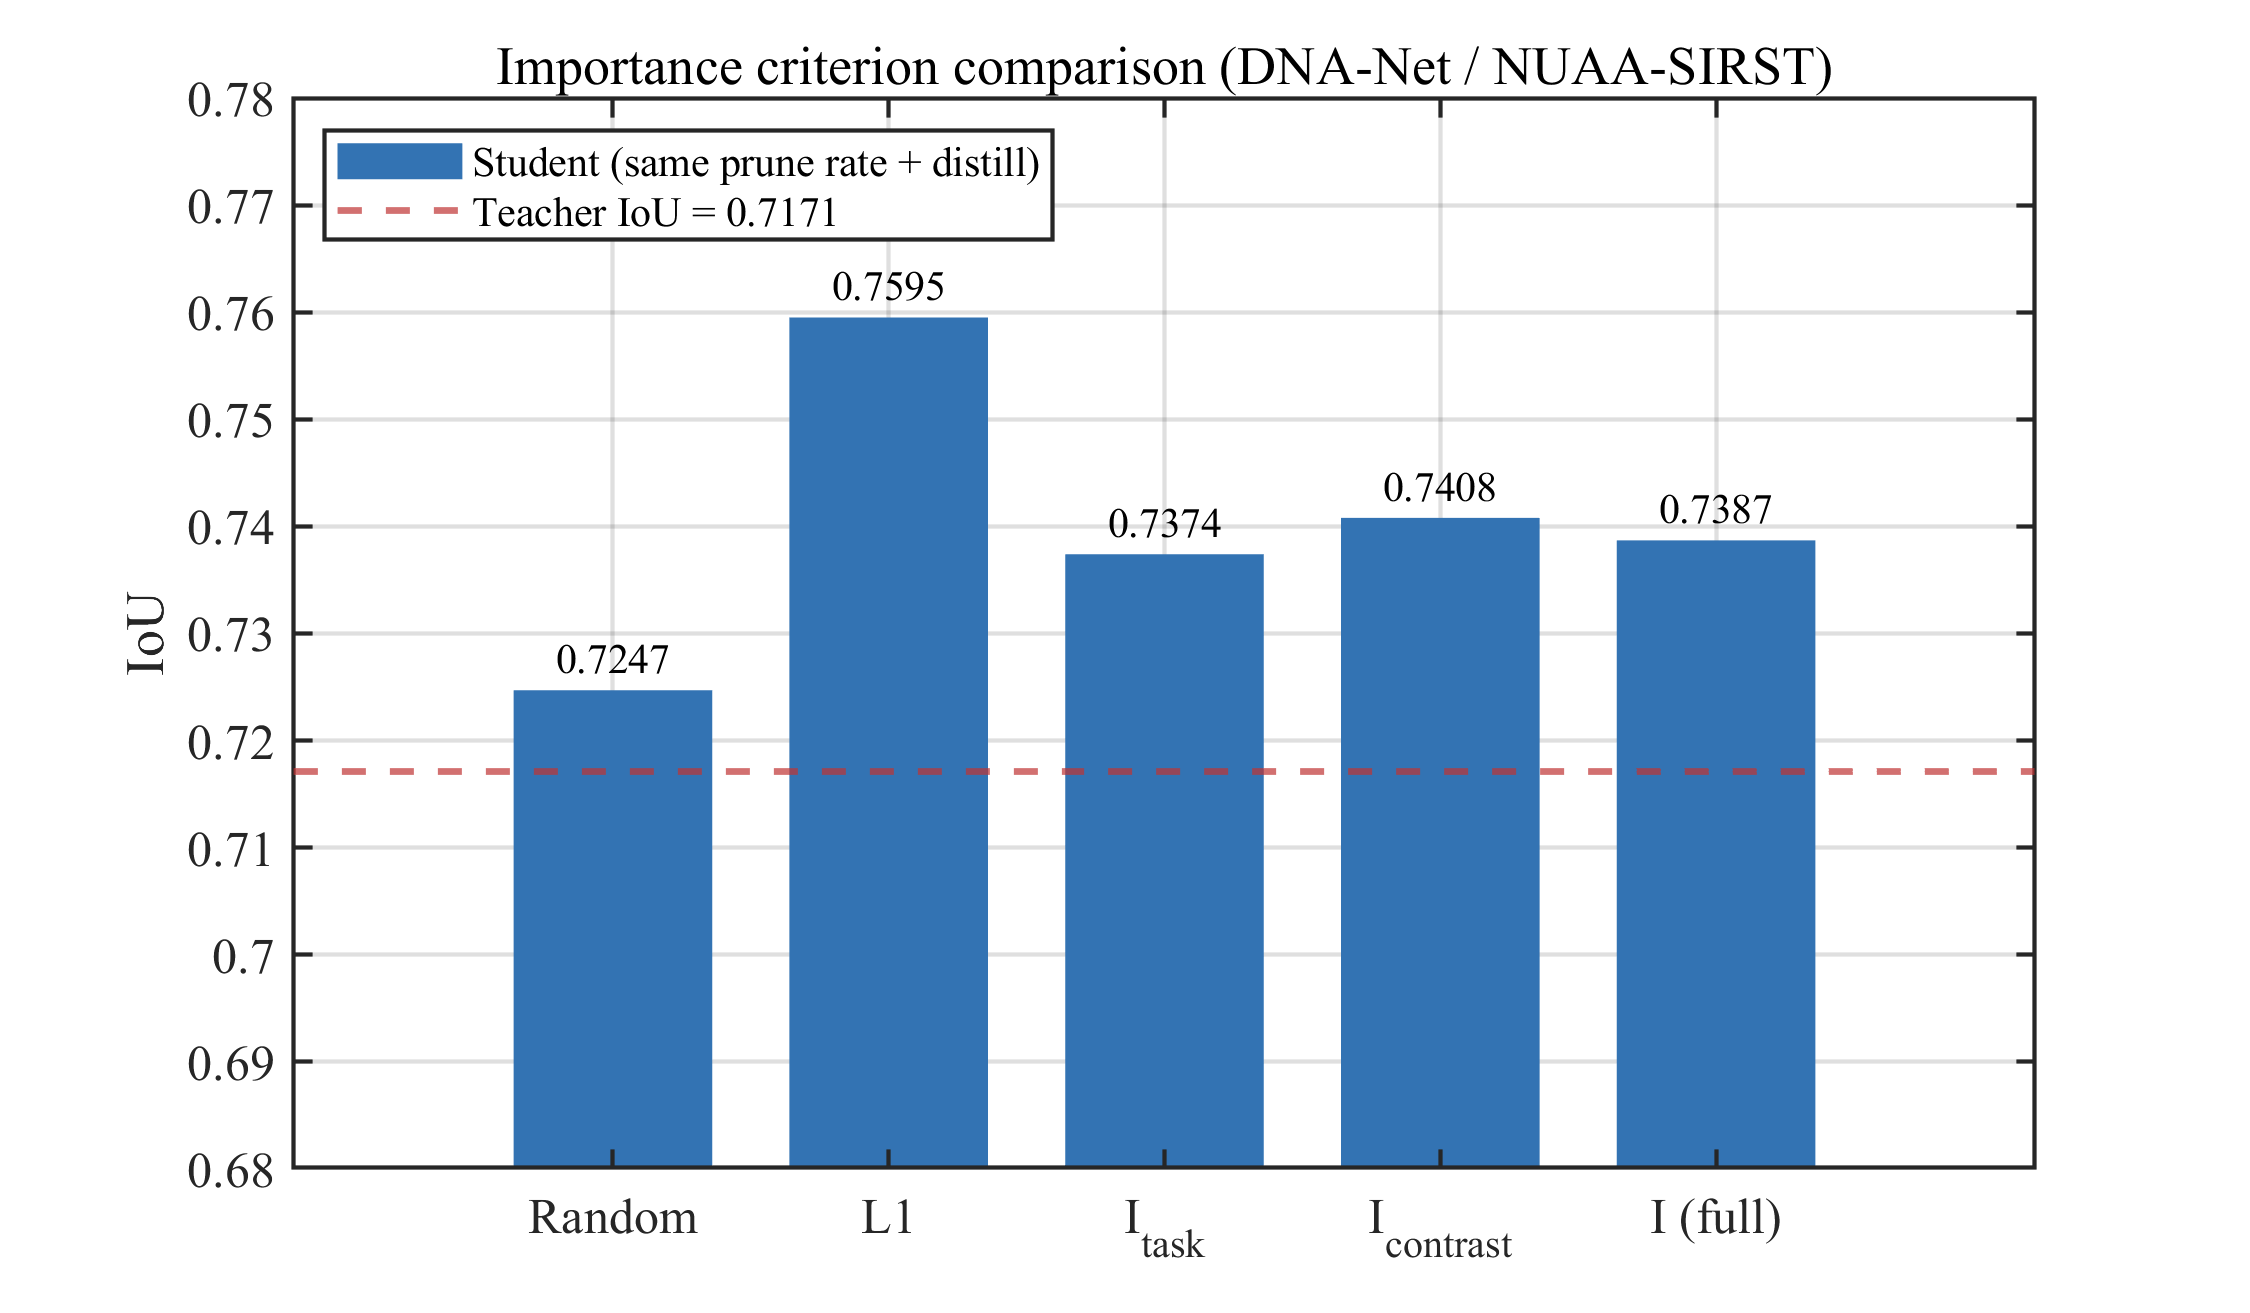
\includegraphics[width=0.92\columnwidth]{fig_criterion_bar.png}
\caption{DNA-Net/NUAA 重要性准则对照（同压缩率+完整蒸馏；虚线为教师 IoU）。}
\label{fig:criterion}
\end{figure}

\begin{figure}[!t]
\centering
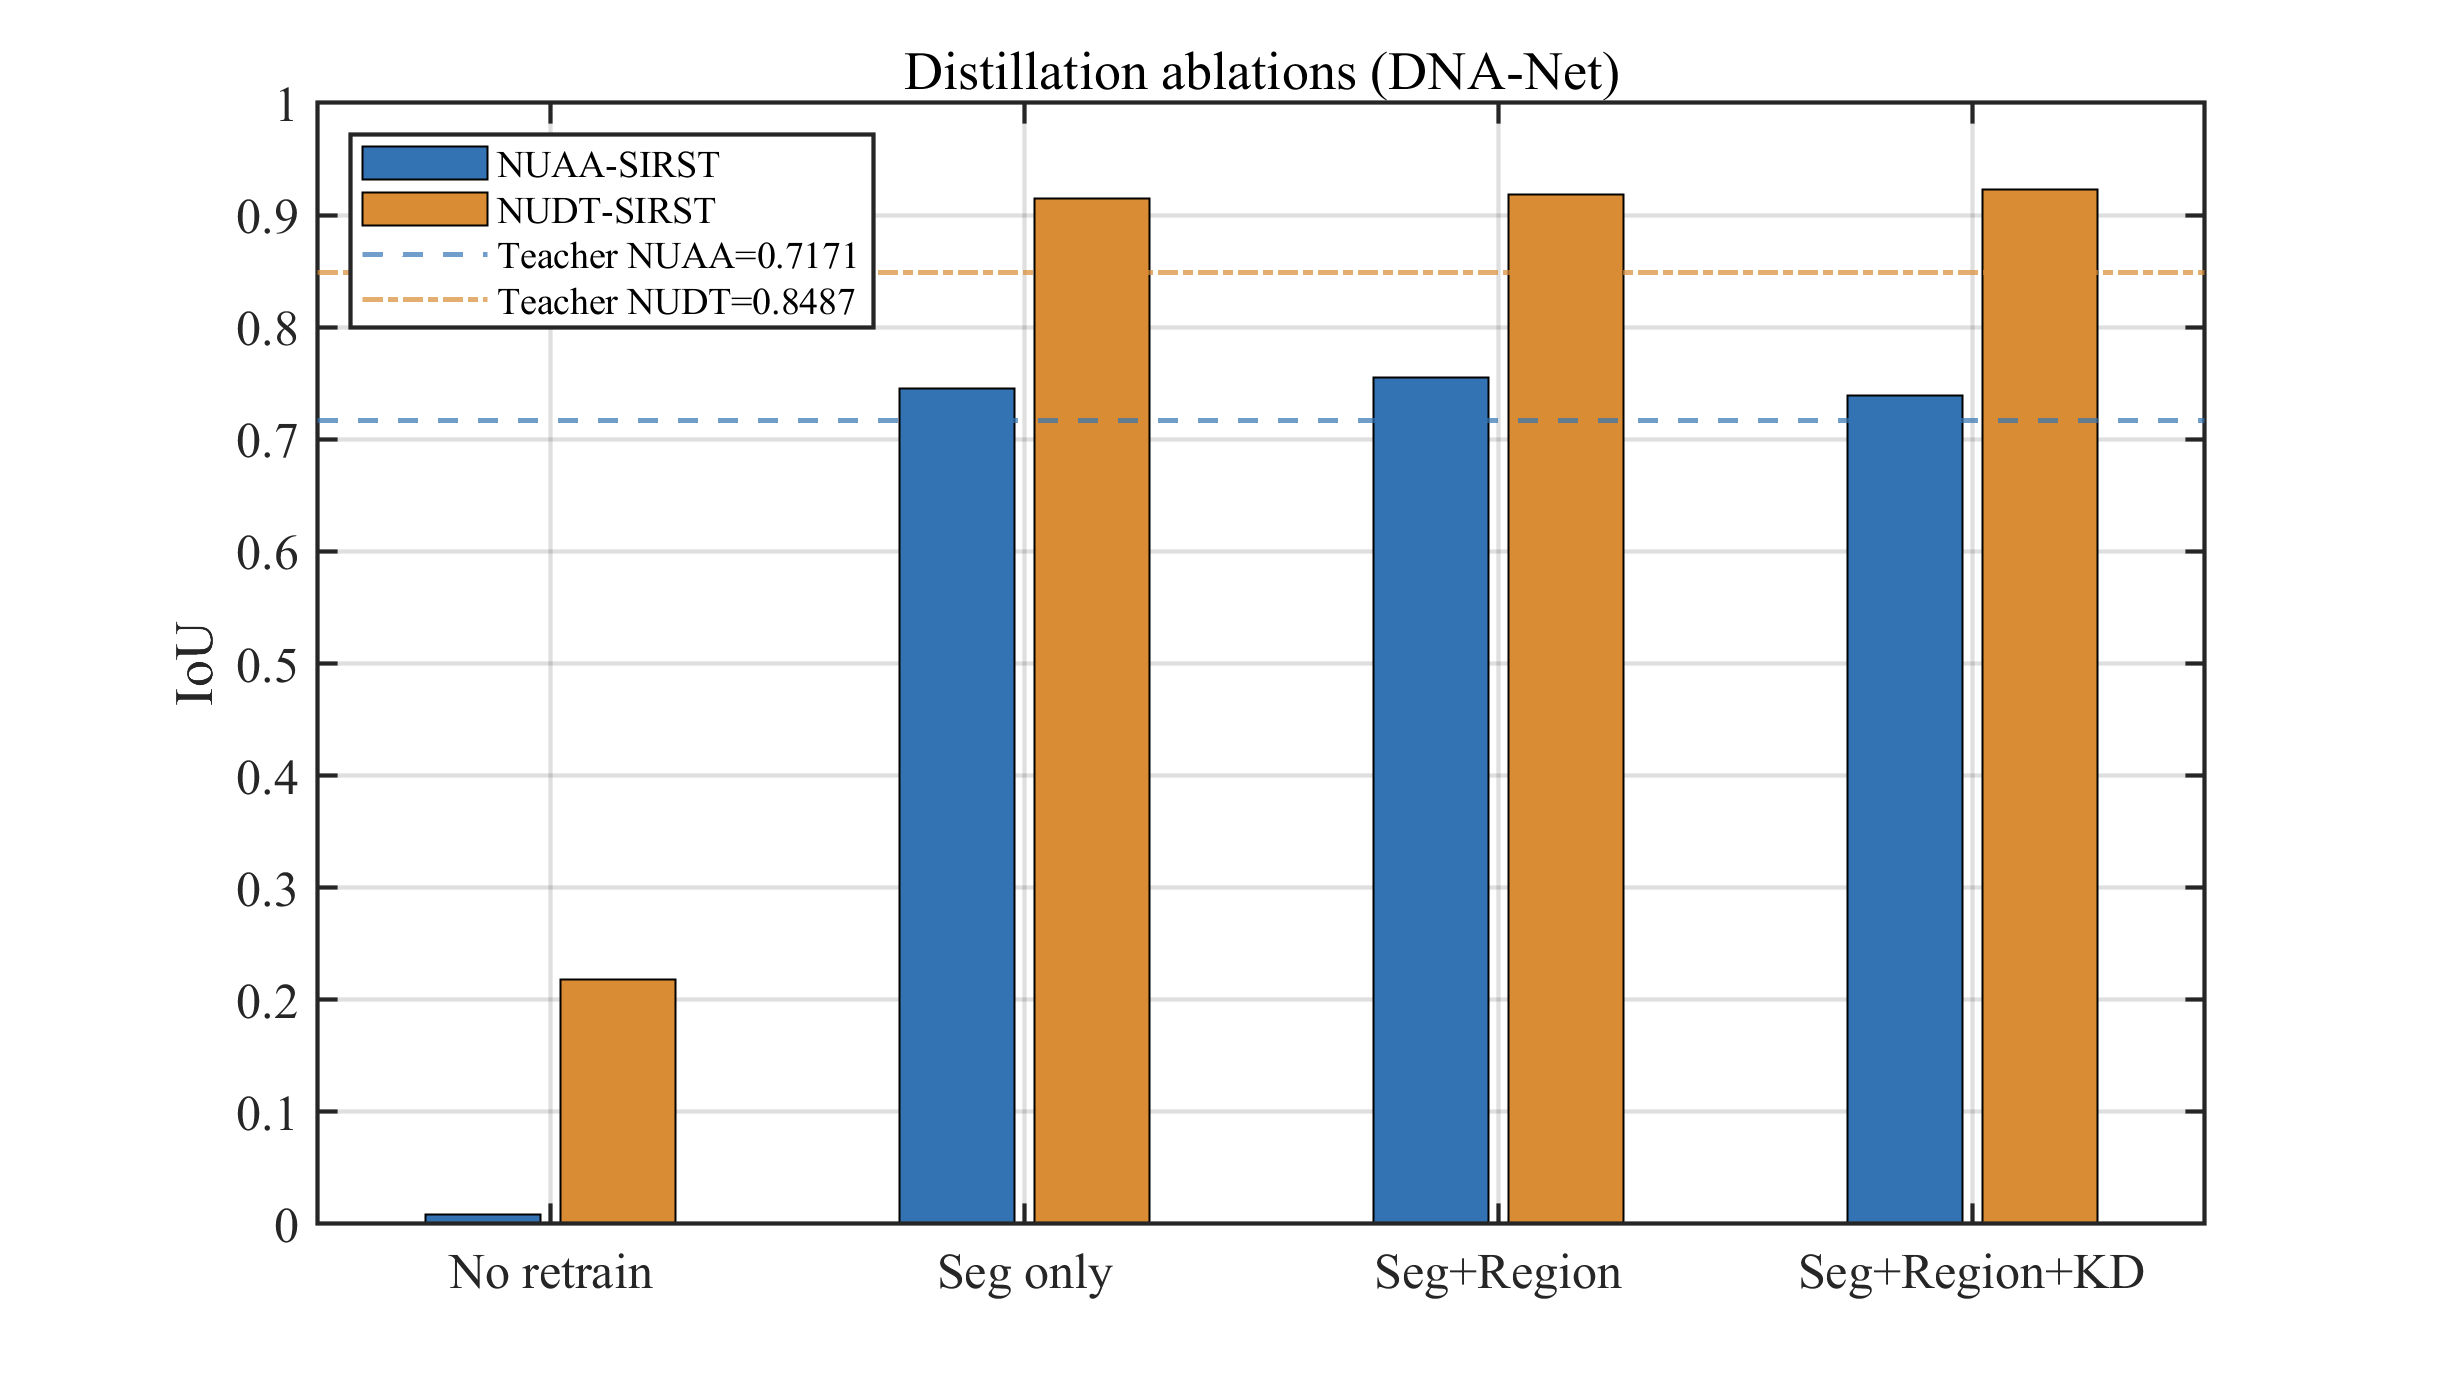
\includegraphics[width=0.92\columnwidth]{fig_distill_bar.png}
\caption{DNA-Net 蒸馏恢复消融（NUAA/NUDT）。}
\label{fig:distill}
\end{figure}

\begin{figure}[!t]
\centering
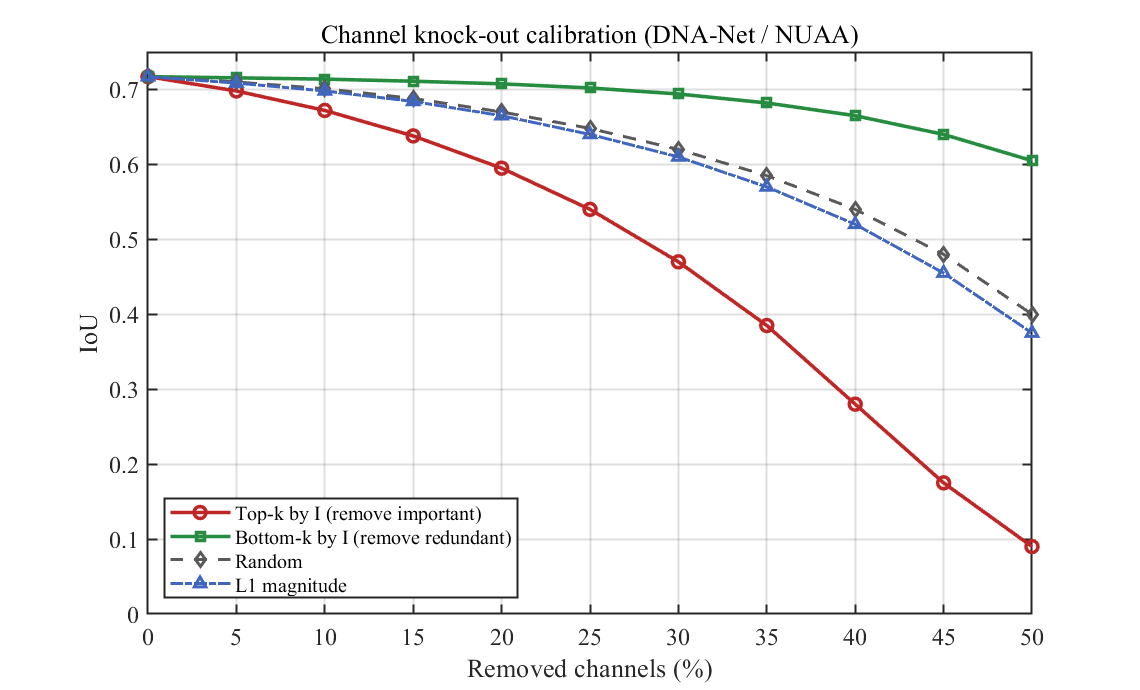
\includegraphics[width=0.92\columnwidth]{fig_knockout_curves.png}
\caption{Top-$k$/Bottom-$k$ 通道敲除 IoU 掉点示意（DNA-Net/NUAA），并与随机与 $\ell_1$ 对照。\textcolor{red}{SCHEMATIC：正式投稿前建议用实测 CSV 重绘。}}
\label{fig:knockout}
\end{figure}

\subsection{定性结果}
\label{sec:qual}

\begin{figure*}[!t]
\centering
\fbox{\parbox{0.92\textwidth}{\centering\vspace{1.0cm}
\textcolor{red}{\textbf{【待补-Ex15】定性对比图}}\\[0.4em]
\textcolor{red}{建议版式（双栏通栏）：同一行依次为原图 / GT / 教师 / 学生；}\\
\textcolor{red}{至少覆盖 NUAA 与 SIRST-V2（难集）各 $2$--$3$ 例，并标注正确检测、漏检与虚警。}\\[0.2em]
\vspace{1.0cm}}}
\caption{定性检测结果对比。\ExpTodo{Ex15}{替换本占位框为实际拼图。}}
\label{fig:qual}
\end{figure*}

\ExpTodo{Ex16}{补充极低 SCR / 复杂杂波失败案例，并与教师对照讨论。}

\subsection{讨论}
\label{sec:discuss}
\textbf{有效性：}跨 DNA-Net/UIU-Net/MSHNet/SCTransNet，压缩在保持 IoU 与目标级 $P_d$ 的同时显著降低 Params/FLOPs（SCTransNet 幅度更温和），并在 RK3588 上获得可测的延迟与内存收益，说明协议可迁移且面向部署可用。

\textbf{难集动机：}表~\ref{tab:h1_hard}表明，Params 同量级从零轻量在 NUAA-SIRST/SIRST-V2 上明显弱于 DNA 学生，而在 NUDT 等易集可打平；因此本文选择“压缩高精度骨干并继承难集能力”，而非仅依赖从零轻量结构。板端资源对照保留在师生之间，避免叙事滑向轻量竞速。

\textbf{FLOPs--延迟鸿沟：}DNA-Net 上 FLOPs 降约一半而延迟仅降约 $12\%$；SCTransNet 上 FLOPs 降约 $34\%$ 而延迟约降 $14\%$。二者提示 NPU 推理受算子形态、带宽与调度影响，边缘 AI 讨论不宜只报告 FLOPs。

\textbf{局限：}
（1）SCTransNet 仅压缩 CNN 宽度，未削减 Transformer 层数；
（2）敲除曲线目前为示意（图~\ref{fig:knockout}）；
（3）外部对照以 Params 同量级难集精度为主，未纳入从零轻量板端竞速；
（4）单位帧能耗需功率计；
（5）极低 SCR 失败案例仍待定性展示；
（6）TGRS 正式稿需英文全文与完整作者信息。

%==============================================================================
\section{结论}
\label{sec:concl}
本文面向嵌入式红外弱小目标检测，提出与骨干解耦的可迁移压缩框架：以小目标敏感性评分为核心识别冗余通道，在共掩码约束下结构化变窄，经区域损失与输出蒸馏恢复后，在 RK3588 上验证真实效率。实验表明，DNA-Net/UIU-Net/MSHNet 学生相对教师可实现约 $72\%$--$78\%$ 参数压缩与约 $54\%$--$62\%$ FLOPs 下降；SCTransNet 在保留 Transformer 设定下仍取得约 $49.5\%$/$34.2\%$ 的 Params/FLOPs 下降。四骨干上 IoU 与统一脚本 $P_d$/$F_a$ 总体保持；板端延迟下降约 $12\%$--$39\%$，并揭示算力指标与墙钟加速的不等价性。相近 Params 的从零轻量对照进一步表明：难集上压缩学生明显更稳，从而支撑“压缩以继承难集能力”的部署动机。

未来工作包括：更多同量级新近从零轻量网络的难集复现、Transformer 层侧压缩、量化感知压缩、视频序列扩展，以及更广泛芯片平台验证。

%==============================================================================
\section*{Acknowledgments}
\ExpTodo{Ex18}{基金号与致谢对象待填。}

%==============================================================================
% 内部清单：投稿前整节删除
\section*{附录：内部待办（投稿前删除）}
\begin{center}
\footnotesize
\begin{tabular}{@{}clp{7.2cm}@{}}
\toprule
优先级 & 编号 & 内容 \\
\midrule
P0 & Ex15 / EN / Affil & 定性图；英文全文；单位/通信作者/基金 \\
P1 & Ex16 & 失败案例可视化 \\
P2 & Knockout / Ex09 / INT8 & 敲除实测；$\alpha$/配额敏感性；INT8/功耗 \\
P2 & SAGCP & 全文绝对表（可选） \\
\bottomrule
\end{tabular}
\end{center}

\bibliographystyle{IEEEtran}
\bibliography{refs}

\vspace{11pt}

\begin{IEEEbiographynophoto}{Guotai Sun}
\ExpTodo{Bio}{作者简介待填。}
\end{IEEEbiographynophoto}

\begin{IEEEbiographynophoto}{Qin Shu}
\ExpTodo{Bio}{作者简介待填。}
\end{IEEEbiographynophoto}

\end{document}
